% !TEX encoding = UTF-8
%Koma article
\documentclass[fontsize=12pt,paper=letter,twoside]{scrartcl}
\usepackage{float}
\usepackage{listings}
\usepackage{makecell}

%Standard Pre-amble
\usepackage[top=4cm,bottom=4cm,left=3cm,right=3cm,asymmetric]{geometry}
%\geometry{landscape}                % Activate for for rotated page geometry
%\usepackage[parfill]{parskip}    % Begin paragraphs with an empty line rather than an indent
\usepackage[table,xcdraw]{xcolor}
\usepackage{graphicx}

\usepackage{amsmath}
\usepackage{amssymb}
\usepackage{epstopdf}
\DeclareGraphicsRule{.tif}{png}{.png}{`convert #1 `dirname #1`/`basename #1 .tif`.png}
% Listings needs package courier
\usepackage{listings} % Needs 
\usepackage{courier}

\usepackage[framemethod=TikZ]{mdframed}
\usepackage{url}

\usepackage{sty/bsymb} %% Event-B symbols
\usepackage{sty/eventB} %% REQ and ENV
\usepackage{sty/calculation}

%Maths
\usepackage{amssymb,amsmath}
\def\Fl{\mathbb{F}}
\def\Rl{\mathbb{R}}
\def\Nl{\mathbb{N}}
\def\Bl{\mathbb{B}}
\def\St{\mathbb{S}}
\newcommand{\ovr}{\upharpoonright}
\newcommand{\var}[1]{\textit{#1}}
%Useful definitions
\newcommand{\mv}[1]{\textit{m\_#1}}
\newcommand{\cv}[1]{\textit{c\_#1}}
\newcommand{\degree}[1]{^{\circ}\mathrm{#1}}
%\newcommand{\comment}[1]{{\footnotesize \quad\texttt{--}\textrm{#1}}}
\newcommand{\im}[1]{i\texttt{-\!#1}}

\usepackage[headsepline]{scrpage2}
\pagestyle{scrheadings}
\ihead[]{\small EECS4312 Report1}
\ohead[]{\small \thepage}
\cfoot[]{}
\ofoot[]{}


%%%%PVS environment%%%%%%%%%%%%%%%%%%%
\lstnewenvironment{pvs}[1][]
    {\lstset{#1,captionpos=b,language=pvs,
    mathescape=true,
    basicstyle=\small\ttfamily,
    numbers=none,
    frame=single,
    % numberstyle=\tiny\color{gray},
    % backgroundcolor=\color{lightgray},
    firstnumber=auto
    }}
    {}
 %%%%%%%%%%%%%%%%%%%%%%%%%%%%%%%%
 
%%%%Verbatim environment%%%%%%%%%%%%%%%%%%%
\lstnewenvironment{code}[1][]
    {\lstset{#1,captionpos=b,
    mathescape=true,
    basicstyle=\small\ttfamily,
    numbers=none,
    frame=single,
    % numberstyle=\tiny\color{gray},
    % backgroundcolor=\color{lightgray},
    firstnumber=auto
    }}
    {}

% \newenvironment{boxed}[1]
%    {\begin{center}
%    #1\\[1ex]
%    \begin{tabular}{|p{0.9\textwidth}|}
%    \hline\\
%    }
%    { 
%    \\\\\hline
%    \end{tabular} 
%    \end{center}
%    }
 %%%%%%%%%%%%%%%%%%%%%%%%%%%%%%%%
 
 %Text in a box
\newenvironment{textbox}
    {\begin{center}
    \begin{tabular}{|p{0.9\textwidth}|}
    \hline\\
    }
    { 
    \\\\\hline
    \end{tabular} 
    \end{center}
    }

\usepackage{hyperref}

%Highlight \hl{}
\usepackage{soul}

\usepackage{enumitem}
\newlist{mylist}{itemize}{1}
\setlist[mylist]{label=\textbullet,leftmargin=1cm,nosep}

\usepackage{multirow}

% Reduce space between figure and caption
%\usepackage{caption}
%\captionsetup[table]{font=small,skip=0pt}     %% Adjust here
%or equivalently 
\usepackage[font=small,skip=4pt]{caption}
%Useful definitions
%\newcommand{\mv}[1]{\textit{m\_#1}}
%\newcommand{\cv}[1]{\textit{c\_#1}}
%\newcommand{\degree}[1]{^{\circ}\mathrm{#1}}
%\newcommand{\comment}[1]{{\footnotesize \quad\texttt{--}\textrm{#1}}}

% Set the header
\ihead[]{\small EECS4313 Assignment-2}


%%%%%%%%%%%%Enter your names here%%%%%%%%
\author{Student Name | Student Number | EECS Account
\and \textbf{Edward Vaisman | 212849857 | eddyv}
\and \textbf{Robin Bandzar | 212200531 | cse23028}
\and \textbf{Kirusanth Thiruchelvam | 212918298 | kirusant}
\and \textbf{Sadman Sakib Hasan | 212497509 | cse23152}
}
%%%%%%%%%%%%%%%%%%%%%%%%%%%%%%%%

\date{\today} % Display a given date or no date

\begin{document}
\title{EECS 4313 Assignment 2 \\Black-box and White-box Testing with JUnit}
\maketitle

\newpage

%%%%%%%%%%%%%%%%%%%%%%%%%%%%%%%
\tableofcontents


\newpage


%%%%Rest of your document goes here%%%%%%%%%%%%%%%%%%%

\section{Black Box Testing}

\subsection{Boundary Value Testing}

\begin{itemize}
\item Specification of the selected Java methods.
\item Justification of the testing technique chosen, i.e., why is it appropriate for this method.
\item Description of your application of the three testing strategies. Be clear about which test cases
you implemented.
\item Evaluation of the test cases derived by the testing technique. Include the screenshots of the
test running results. If you had to complement the derived test cases with special value 
testing, describe that as well. The marker will not read your code in order to see what you
tested. You have to describe it.
\item Attaching bug reports if bugs are discovered using your testing methods. You should use the
same bug report format as in Assignment 1. Do not file these bug reports to the project’s bug
report system. 
\end{itemize}

\newpage
\subsection{Equivalence Class Testing}

\begin{itemize}
\item Specification of the selected Java methods.
\item Justification of the testing technique chosen, i.e., why is it appropriate for this method.
\item Description of your application of the three testing strategies. Be clear about which test cases
you implemented.
\item Evaluation of the test cases derived by the testing technique. Include the screenshots of the
test running results. If you had to complement the derived test cases with special value 
testing, describe that as well. The marker will not read your code in order to see what you
tested. You have to describe it.
\item Attaching bug reports if bugs are discovered using your testing methods. You should use the
same bug report format as in Assignment 1. Do not file these bug reports to the project’s bug
report system. 
\end{itemize}

\newpage
\subsection{Decision Table Testing}

\begin{itemize}
\item \textbf{Technique}: \emph{Decision Table Testing}
\item \textbf{Class}: \emph{net.sf.borg.common.DateUtil.java}
\item \textbf{Method}: \emph{isAfter(Date d1, Date d2)}
\item \textbf{Method description}: The method checks if a given date \emph{d1} falls on a later calendar day than date \emph{d2}. It returns \textbf{true} if \emph{d1} does fall on a later calendar day than \emph{d2} and \textbf{false} otherwise.
\begin{itemize}
\item \textbf{d1} - The first argument is of type Java Date Object.
\item \textbf{d2} - The second argument is of type Java Date Object.
\end{itemize}
\item \textbf{Justification}: Decision table testing technique is an appropriate testing technique for this method because there are decision making to be done among the input variables. It consists of logical relationships among the input variables, i.e date \emph{d1} appearing before, after or at the same time as date \emph{d2}, which directly affects the output.
\end{itemize}

\begin{table}[h]
\centering
\begin{tabular}{|c | c | c | c | c | c | c | c |}
	\cline{1-8}
	& \textbf{Rule 1-2} & \textbf{Rule 3} & \textbf{Rule 4} & \textbf{Rule 5} & \textbf{Rule 6} & \textbf{Rule 7} & \textbf{Rule 8}\\ \hline
	C1: d1 $<$ d2 & T & T & T & F & F & F & F \\ \hline
	C2: d1 $=$ d2 & T & F & F & T & T & F & F \\ \hline
	C3: d1 $>$ d2 & - & T & F & T & F & T & F \\ \Xhline{2pt}
	A1: Date is after & & & & & & X & \\ \hline
	A2: Date is not after & & & X & & X & & \\ \hline
	A3: Impossible & X & X & & X & & & X \\ \hline
\end{tabular}
\caption {Decision Table for the isAfter method}
\label{tbl:trace_matrix}
\end{table}

\noindent \textbf{Rationale}: The decision table above outlines 8 rules. The rules are derived from three equivalence classes: d1 is less than d2, d1 is equal to d2 and d1 is greater than d2. Each equivalence class can have 2 different values (i.e T or F), giving us $2^3 = 8$ rules. Out of the 8 rules, 5 of the rules points to \emph{Impossible} cases, hence cannot be converted to test cases. The other 3 rules are converted into test cases. Below is the code snippet and the test run screenshot for the test cases derived using the decision table technique.

\newpage
\begin{code}
	@Test
	public void testIsAfter() {
		/** Method used: Decision Table Testing **/
		
		Date d1 = new Date(117, 11, 3);
		Date d2 = new Date(117, 11, 3);
		boolean result;
		
		// date d1 is equal to d2
		result = DateUtil.isAfter(d1, d2);
		assertFalse("Date d1 is equal to d2", result);
		
		// date d1 is before d2
		d1.setDate(2);
		result = DateUtil.isAfter(d1, d2);
		assertFalse("Date d1 is before d2", result);
		
		// date d1 is after d2
		d1.setDate(4);
		result = DateUtil.isAfter(d1, d2);
		assertTrue("Date d1 is after d2", result);
	}
\end{code}

\begin{figure}[!htb]
\begin{center}
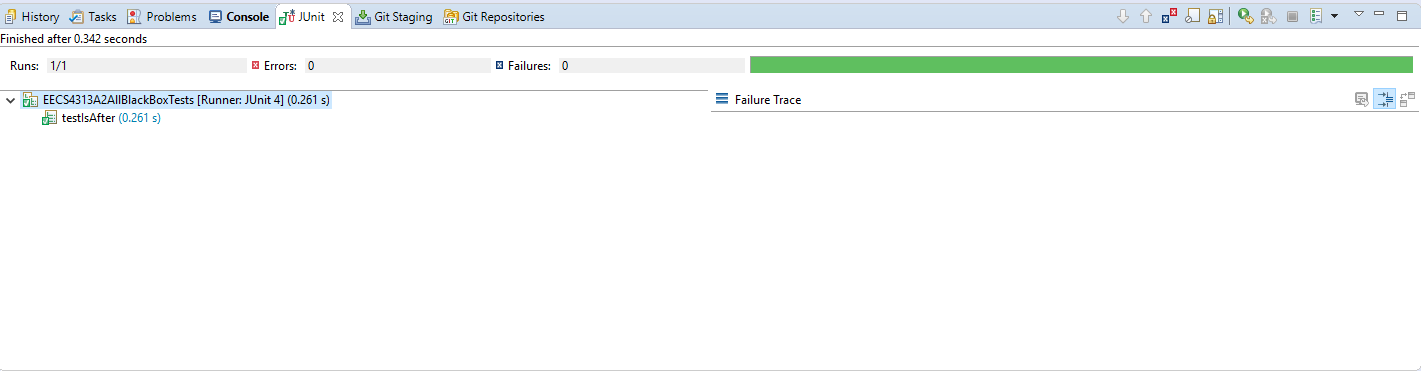
\includegraphics[width=.99\textwidth]{images/bbt/dtt.png}
\end{center}
\caption{Test results using Decision Table Testing Technique}
\label{fig:bbt_dtt}
\end{figure}

\newpage
\section{White Box Testing}

\begin{itemize}
\item The statement coverage measurements for your Assignment 2 test suite.
\item A description of the test cases that you added in this assignment to improve statement
coverage. The marker will not read your code in order to see what you tested. You have to
describe it.
\item The statement coverage measurements for your final submission. Include the screenshots of
the test running results and the screenshots of the coverage measurement. If your coverage is
not 100%, include a discussion on why that is.
\item The Control Flow Graph you created. Indicate the segments clearly (you will probably need
to include the code for this).
\item The path coverage discussion described in section 2 above.
\item Attaching bug reports if bugs are discovered using your testing methods. You should use the
same bug report format as in Assignment 1. Do not file these bug reports to the project’s bug
report system.
\item An appendix with the specification of the methods you are testing (if there are new ones). 
\end{itemize}

\end{document}
